
\subsection{Échanger pions et dames à changement de joueur}

Dans cette section, nous avons ajouté une option qui nous permet d'avoir le choix d'échanger 
des jetons noirs et blancs en pions ou dames.


\begin{figure}[hp]
	      \begin{center}
			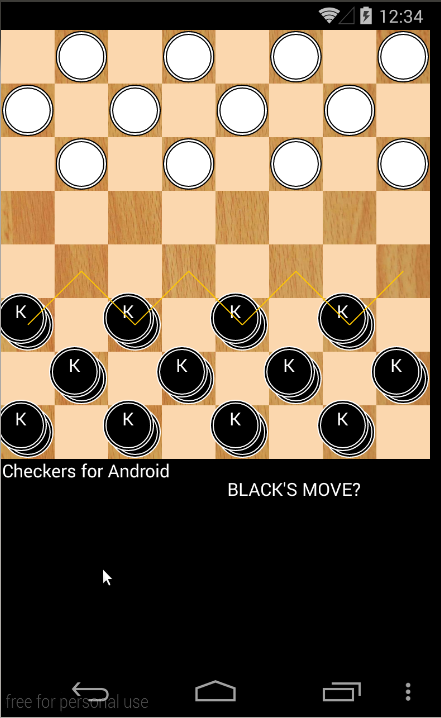
\includegraphics[width=0.4\textwidth]{state0}
	      \end{center}
	\caption{Avant modification}
\end{figure}
Pour celà nous avons d'abord ajouté une option "Switcher les Dames" dans le menu "Options". 
\begin{figure}[h!]
	      \begin{center}
			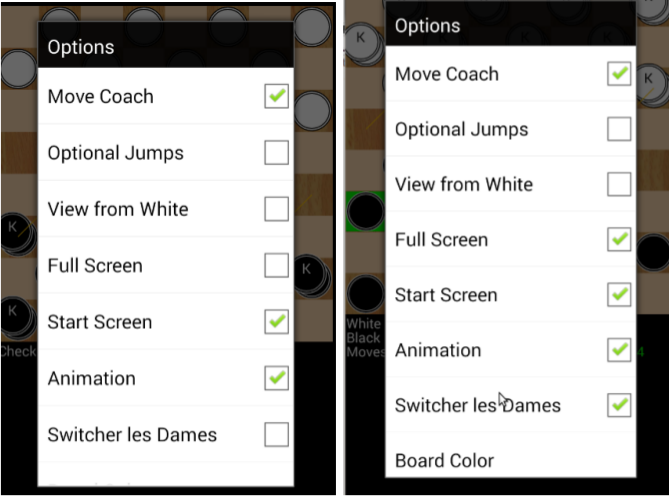
\includegraphics[width=0.8\textwidth]{menu}
		  \end{center}
	\caption{ajout d'une option dans le menu}
\end{figure}
On a effectué cet ajout dans \textit{Chechers.smali} comme on peut le voir sur la Figure 9.\newpage

\begin{figure}[h!]
\begin{verbatim}
    const/4 v1, 0x6
    const/4 v2, 0x6
    const-string v3, "Switcher les Dames"
    invoke-interface {v0, v4, v1, v2, v3}, Landroid/view/SubMenu;->
        add(IIILjava/lang/CharSequence;)Landroid/view/MenuItem;
    move-result-object v1
    invoke-interface {v1, v4}, Landroid/view/MenuItem;->
        setCheckable(Z)Landroid/view/MenuItem;
    move-result-object v1
    iget-object v2, p0, Lcom/xxogli/xadroid/checkers/Checkers;->
        a:Lcom/xxogli/xadroid/checkers/b;
    invoke-virtual {v2, v5}, Lcom/xxogli/xadroid/checkers/b;->
        permuter(Z)Z
    move-result v2
    invoke-interface {v1, v2}, Landroid/view/MenuItem;->
        setChecked(Z)Landroid/view/MenuItem;
    \end{verbatim}
    \caption{Ajout de l'Option dans onCreateOptionsMenu}
\end{figure}


Après avoir ajouté l'option "Switcher les Dames" dans le menu des Options, nous insérons la méthode permuter() qui prend 
un booléen en paramètre et qui renvoie l'état de la variable \textbf{switchdame} qui est un attribut de la "classe b" de type booléen que nous avons ajouté.


\begin{figure}[!hp]
\begin{verbatim}
.method public final  permuter(Z)Z
.locals 1
    if-eqz p1, :cond_0
    iget-boolean v0, p0, Lcom/xxogli/xadroid/checkers/b;->switchdame:Z
    if-eqz v0, :cond_1
    const/4 v0, 0x0
    :goto_0
    iput-boolean v0, p0, Lcom/xxogli/xadroid/checkers/b;->switchdame:Z
    :cond_0
    iget-boolean v0, p0, Lcom/xxogli/xadroid/checkers/b;->switchdame:Z
    return v0
    :cond_1
    const/4 v0, 0x1
    goto :goto_0
.end method
\end{verbatim}
    \caption{Ajout de l'action dans onCreateOptionsMenu}
\end{figure}

Nous avons ensuite ajouté l'action à exécuter lorsqu'on choisit l'option "Switcher les Dames" dans \textit{onOptionsItemSelected}.

\begin{figure}[!hp]
\begin{verbatim}
    :cond_9
    const/4 v2, 0x6
    if-ne v1, v2, :cond_10
    iget-object v1, p0, Lcom/xxogli/xadroid/checkers/Checkers;->
        a:Lcom/xxogli/xadroid/checkers/b;
    invoke-virtual {v1, v0}, Lcom/xxogli/xadroid/checkers/b;->
         permuter(Z)Z
    move-result v1
    invoke-interface {p1, v1}, Landroid/view/MenuItem;->
        setChecked(Z)Landroid/view/MenuItem;
    goto/16 :goto_0
\end{verbatim}
    \caption{Ajout de l'action dans le onOptionsItemSelected}
\end{figure}

\newpage

Le résultat est affiché comme suit.

\begin{figure}[h!]
	      \begin{center}
			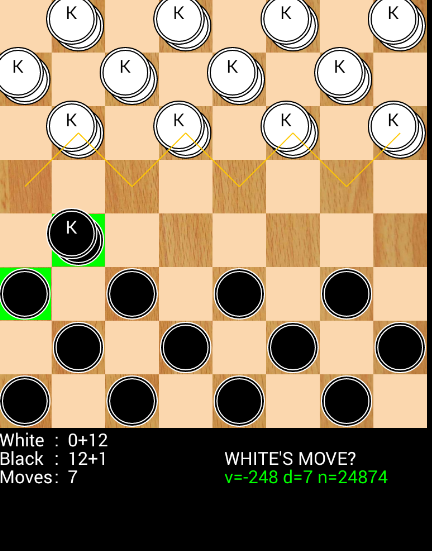
\includegraphics[width=0.4\textwidth]{state1}
	      \end{center}
	\caption{avant modification}
\end{figure}


\paragraph{Remarque:}
Lors de l'execution, nous avons constaté qu'il y avait un soucis avec la permutation.
Ce dernier est dû au au fait que le contrôleur doit prévoir à l'avance le coup qu'il va jouer en fonction
de la position des jetons qu'il a avant d'effectuer le switch.
Ainsi, on se retrouve avec un jeton supplémentaire de l'ancien type.

